\chapter{Quasiparticle Interference (QPI)}
%todo: to write the abstract of this chapter after finishing this chapter
%todo: to standardize the vector form in this chapter 
\section{Introduction to Quasiparticle Interference measurement}

\subsection{Terminology}
To set stage for the discussion in this chapter, we must make distinctions between the following terminologies: 
\begin{itemize}
	\item \ac{QPI}: a physical phenomenon describing the interference of all possible quasiparticles, a concept used to describe the collective behavior of a group of particles. examples of quasiparticle excitation include phonon in crystalline solids, Bogoliubov quasiparticle in superconductors etc. 
	\item QPI pattern: a pattern that can be observed in different physical system that corresponds to the physical phenomenon QPI.
	\item QPI measurement: a measurement that measures the QPI patterns presented in systems that intrinsically host QPI.
\end{itemize}
We should note that STM is not the only tool that can perform QPI measurement. In fact, interference of quasiparticles are reported across a wide literature in different systems using different techniques. For example,
%todo: to wirte different examples here, template as X used Y technique to detect G quasiparticle Interference pattern in Z system.: ranging from crystalline excitation like phonon in Si phononic crystals \cite{maldovan_phonon_2015}, electronic excitation like Bogoliubov quasiparticle in superconductors interference strongly\cite{homan_search_nodate}

I will then elaborate what these terms mean in the context of STM study, and to reduce redundancy, in the following writing, QPI, QPI pattern and QPI measurement will be referred specifically to STM studies.

\subsection{what is QPI measurement in STM studies}
In a word. QPI measurement is an STM technique that aims to probe the band structure of a material by studying QPI patterns presented on the surface of a material. 

Imagine an ideal metal with no crystal imperfection, with Landau's Fermi liquid theory, we know that the Landau quasiparticle has an eigenstate described by a Bloch wavefunction: 

\begin{equation}
\psi(\mathbf{r}) = e^{i \mathbf{k} \cdot \mathbf{r}} u(\mathbf{r})
\label{eq:bloch}
\end{equation} 
where $k$ is the crystal momentum of the quasiparticle. And the electron \ac{LDOS} can be written as  
\begin{equation}
\text{LDOS}(E, \vec{r}) \propto \sum_k |\Psi_k(\vec{r})|^2 \delta(E - \varepsilon(k))
\label{eq:ldos}
\end{equation}

where  $\epsilon(k)$ is the energy dispersion of the Bloch state for different $\vec{k}$. And if we plug Equation (\ref{eq:bloch}) into Equation (\ref{eq:ldos}), we see that $\text{LDOS}$ is translationally invariant at all Bravais-lattice-equivalent points. Thus why in ideal case, real space imaging technique like \ac{STM}, can not be used to measure $\epsilon(k)$. 

However, crystal imperfections as discussed in Ch.4 can help us introduce a momentum texture to the $\text{LDOS}(E, \vec{r})$. In low temperature STM, where the phonon modes and other excitation are rare or absent, lattice imperfections such as point defects can cause elastic scattering which mixes electronic eigenstates at different $\vec{k}$ but at the same energy, the interference between the incoming and outgoing wave forms a "standing wave" that act as a real space modulation in $\text{LDOS}(E)$ described as a impurity-induced Friedel oscillation\cite{bena_friedel_2016}. This spatial modulation in $\text{LDOS}$ is the QPI pattern that we refer to in STM studies. We can perform \ac{STS} measurement on the region that presents this QPI pattern, then perform Fourier transformation to the STS, we can observe this QPI pattern in the momentum space. This whole process of detecting QPI pattern and analyze it in momentum space is what we call a QPI measurement. 

We will show case this \ac{LDOS} modulation with a simulation on a toy model in the following section. 

\begin{figure}
	\centering
	\includegraphics[width=0.5\textwidth]{example-image-a} % Replace with your image file
	\caption{Friedel oscillation and QPI}
	\label{fig:example}
\end{figure}

\subsection{LDOS modulation simulation on a square lattice}

As mentioned in last section \ac{QPI} measurement is the Fourier transformed spatial \ac{STS} measurement, which is proportional to the \ac{LDOS}. Thus, to understand \ac{QPI} measurement, we must understand the origin of \ac{QPI} pattern and how it modifies \ac{LDOS}. Here, I present an investigation into the \ac{LDOS} modulation caused by point defects on a square lattice, this textbook exercise is inspired by work from Cheung et al \cite{cheung_dictionary_nodate}.

\subsubsection{Theory}
We first consider a square lattice with lattice constant $a$, and model it through the single-electron \ac{TB} model considering only nearest-neighbor hopping. This hopping is characterized with a fixed negative number $t$ named hopping-parameter. We then place $N_d$ number of defects onto different lattice sites as a perturbation to the \ac{TB} Hamiltonian $H_0$. The total Hamiltonian can then be written as: 
$\hat{H} = \hat{H}_0 + \hat{H}_d$. $\hat{H}_d$ can be written as: 
\[
\hat{H}_d = \sum_{\alpha=1}^{N_d} E_\alpha \lvert \alpha \rangle \langle \alpha \rvert,
\] 
where $\alpha$ enumerates $\alpha^{th}$ defect located at $x_\alpha$, we then write the \ac{TB} Hamiltonian and transfer it into momentum space:
\begin{align}
\hat{H}_0 = E_0 -t \sum_{j,\tau} (c_j^{+} c_{j+\tau} + c_{j+\tau}^{+} c_j) \label{h0_real} \\
\hat{H}_0 = E_0 -\sum_{k} \epsilon_k c_k^{+} c_k \label{h0_k} \\
\epsilon_k = -2t(cos(k_x a)+cos(k_y a)) \label{E_k}
\end{align}
Now we consider our measurable \ac{LDOS} $\rho(\mathbf{x},\omega)$:
\begin{equation}
\rho(\mathbf{x},\omega) = \rho^{0}(\mathbf{x},\omega) - \frac{1}{\pi} \operatorname{Im} \left[ \langle \mathbf{x} | \hat{G}_0 \hat{T} \hat{G}_0 |\mathbf{x} \rangle \right],
\label{ldos}
\end{equation}
where $\hat{G}_0$ and $\hat{T}$ are the \ac{BLGF} and the scattering T-matrix, respectively, according to the pertubative scattering theory. And since we are interested in the modulation of \ac{LDOS} caused by the defects, our actual observable is $\delta \rho(\mathbf{x}, \omega) \equiv \rho(\mathbf{x}, \omega) - \rho^{(0)}(\mathbf{x}, \omega)
$, which is the second term in Equation (\ref{ldos}).
To start, we need to compute the matrix element of \ac{BLGF} $G_0(\mathbf{x},\mathbf{x'},\omega)$:
\begin{align}
	G_0(\mathbf{x},\mathbf{x}';\omega) &= \langle \mathbf{x} | \hat{G}_0(\omega) | \mathbf{x}' \rangle, \\
\end{align}
where
\begin{align}
	\hat{G}_0(\omega) &= \int_{\text{BZ}} \mathrm{d}\mathbf{k} \, \frac{1}{\omega - \hat{H}_0} \lvert \mathbf{k} \rangle \langle \mathbf{k} \rvert \nonumber \\ 
	&= \int_{\text{BZ}} \mathrm{d}\mathbf{k} \, \frac{1}{\omega - E_\mathbf{k}} \lvert \mathbf{k} \rangle \langle \mathbf{k} \rvert.
\end{align}
Then we remind ourselves that in 2D, $\langle \mathbf{k}|\mathbf{x} \rangle = (\frac{1}{\sqrt{2\pi}})^2 e^{-i\mathbf{k}\mathbf{x}}$, and plug the energy dispersion Equation (\ref{E_k}) in, we get: 
\begin{align}
	G_0(\mathbf{x}, \mathbf{x}') = 
	\frac{1}{(2\pi)^2} \frac{1}{2t} 
	\int_{\text{BZ}} \mathrm{d}\mathbf{k} \, 
	\frac{e^{i k_1 (x_1 - x_1')} e^{i k_2 (x_2 - x_2')}}{b - \left( \cos(k_1 a) + \cos(k_2 a) \right)}. 
\end{align}
where $b \equiv \frac{\omega + i\epsilon-E_0}{2t}$ is a dimensionless parameter, we can then define a normalized position deviation $s_j \equiv \frac{1}{a}(x_j-x_j')$ and further reduced the matrix element to its final form: 
\begin{align}
	G_0(\mathbf{x}, \mathbf{x}') = 
	\frac{1}{(2\pi)^2} \frac{1}{2t a^2} 4 \, I_{\text{sq}} 
	\left( \frac{x_1 - x_1'}{a}, \frac{x_2 - x_2'}{a}, b \right) \label{blgf},
\end{align}
where
\begin{align}
	I_{\text{sq}}(s_1, s_2, b) \equiv 
	\int_0^\pi \int_0^\pi \mathrm{d}\phi_1 \, \mathrm{d}\phi_2 \, 
	\frac{\cos(s_1 \phi_1) \cos(s_2 \phi_2)}{b - \cos\phi_1 - \cos\phi_2} \label{Isq}.
\end{align}
Now we proceed to compute the matrix element of T-matrix, we know that: 
\begin{equation}
	\hat{T} = \hat{H_d} (\hat{I} - \hat{G_0}\hat{H_d})^{-1}.
\end{equation} 
And for locations $x_\alpha$, $x_\beta$ on defect sites $\alpha$ and $\beta$, we have: 
\begin{align}
	T_{\alpha\beta} &= \langle \alpha|\hat{H_d} (\hat{I} - \hat{G_0}\hat{H_d})^{-1} | \beta\rangle \\
	&= E_\alpha(\langle \alpha|\hat{I}|\beta\rangle - \langle \alpha|\hat{G_0}\hat{H_d}|\beta \rangle)^{-1} \\
	&= E_\alpha(\delta_{\alpha \beta} - E_\beta G_0(\mathbf{x_\alpha},\mathbf{x_\beta}))^{-1} \label{T_matrix_ele}.
\end{align}
Now with both matrix elements of the \ac{BLGF} and T-matrix, we can finally express $\delta\rho(\mathbf{x},\omega)$ as 
\begin{align}
	\delta\rho(\mathbf{x},\omega) &= - \frac{1}{\pi} \operatorname{Im} \left[ \langle \mathbf{x} | \hat{G}_0 \hat{T} \hat{G}_0 | \mathbf{x} \rangle \right] \\
	&= -\frac{1}{\pi} \operatorname{Im} \left[\sum_{\alpha, \beta=1}^{N_{\text{d}}} G_0(\mathbf{x}, \mathbf{x}_\alpha) T_{\alpha, \beta} G_0(\mathbf{x}_\beta, \mathbf{x})\right].
\end{align}
In single defect case, where $\mathbf{x_\alpha} = \mathbf{x_\beta} = \mathbf{x_d}$, we have: 
\begin{align}
	T(\mathbf{x_d},\omega) &= E_{\text{d}} \left( 1 - E_{\text{d}} G_0(\mathbf{x_d}, \mathbf{x_d}) \right)^{-1} \label{T_matrix_ele} \\
	&= \frac{1}{E_{\text{d}}^{-1} - G_0(\mathbf{x_d}, \mathbf{x_d}; \omega)},
\end{align}
and therefore: 
\begin{align}
	\delta\rho(\mathbf{x},\omega) &= - \frac{1}{\pi} \operatorname{Im}(\frac{(G_0^2(\mathbf{x},\mathbf{x_d};\omega)}{E_d^{-1} - G_0(\mathbf{x_d},\mathbf{x_d};\omega)}) \label{singleldos}. 
\end{align}
And Equation (\ref{singleldos}) can be evaluated numerically with Equation (\ref{blgf}) and Equation (\ref{Isq}).

\subsubsection{Simulation setup}
\begin{figure}
	\centering
	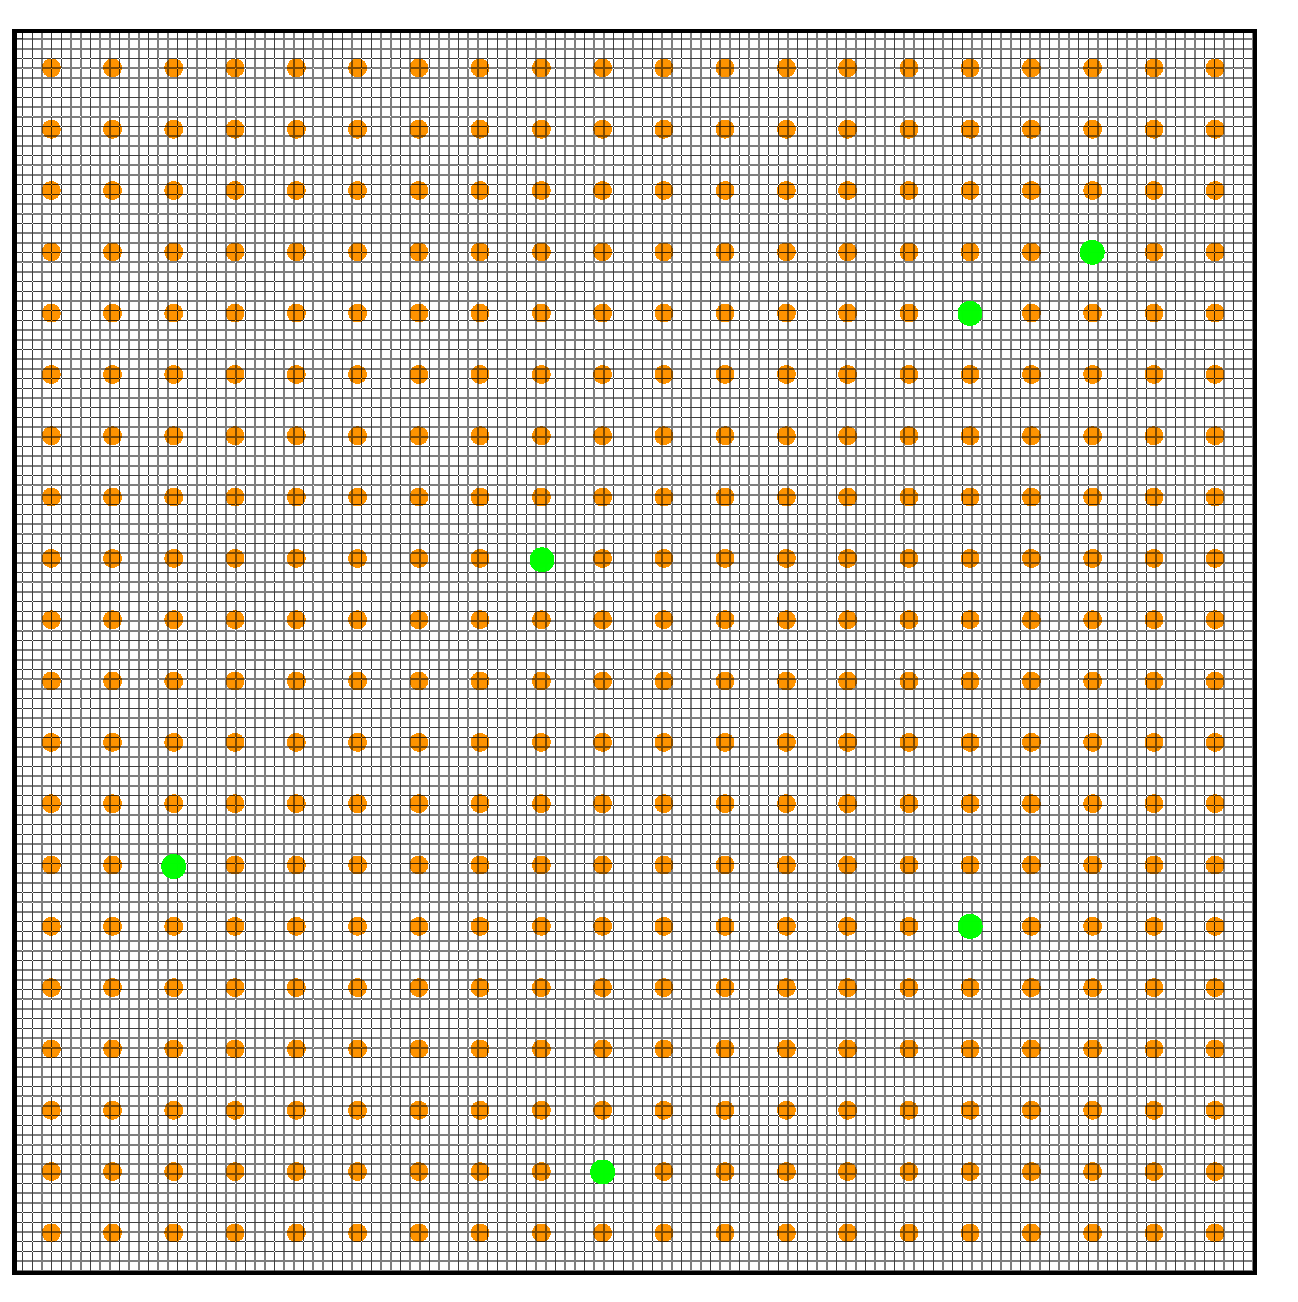
\includegraphics[width=\textwidth]{Ch5_QPIsim_demo.pdf}
	\caption{schematics for the simulation}
	\label{fig:ch5_qpisim_demo}
\end{figure}
\subsubsection{Single defect result}

\subsubsection{Multi defect result}
\begin{itemize}
	\item direct evaluation of $\delta\rho(\mathbf{x},\omega)$
	\item Convolution approach
\end{itemize} 
Estimating the multidefect result with convolution approach inherently makes assumption into the independent nature of scattering, which is only true for weak scattering and sparse impurity distributions. 

\subsubsection{Limitations and assumptions}


\subsubsection{the process}
\subsubsection{the result}


\section{QPI measurements}
How do we measure QPI pattern with STM, the process and analysis we do 
\subsubsection{QPI quality}
Factors determining quality of a QPI measurement, and what is an ideal quality. 
1. high resolution in q-space <-> range in real-space
2. high range in q-space <-> resolution in real-space
3. low noise level-> machine's intrinsic noise level, voltage sweeps and averaging.
4. no phase noise 
\subsubsection{challenges to obtain optimal QPI measurements}
 